\newpage
%\pagenumbering{arabic} % Đánh số thứ tự 1,2,3...
\section*{CHAPTER 2\\ \vspace{0.5cm} CALCULATIONS AND DESIGN}
\addcontentsline{toc}{section}{\numberline{}CHAPTER 2\\ \vspace{0.5cm} CALCULATIONS AND DESIGN}


\begin{table}[H]
    
    \begin{tabular}{l l}
        \fontsize{12pt}{0pt}\selectfont 1. Load: & 
        $ Q_1 =400 \emph{ kg} = 4000\emph{ N} $ \\
        \fontsize{12pt}{0pt}\selectfont 2. Weight of cabinet & 
        G  = 300  \emph{kg} = 3000 \emph{N} \\
         \fontsize{12pt}{0pt}\selectfont 3. Car velocity: & 
        $ V = 10 \emph{ m/min} = 0.167 \emph{ m/s} $ (low speed) \\
        \fontsize{12pt}{0pt}\selectfont 4.	Lifespan: & 
        $ L_h = 16000 $ hours = 4000 \\
         \fontsize{12pt}{0pt}\selectfont 5.	Contact angle between pulley and sheave: & 
        $ \alpha = 137 $ degree  \\
        \fontsize{12pt}{0pt}\selectfont 6.	Distance between two branches of cable:  & 
        $ cc = 1000 $ mm  \\
        \fontsize{12pt}{0pt}\selectfont 7.	Operating condition:  &
        smoothly \\
        \fontsize{12pt}{0pt}\selectfont
        $ Q_m = 2Q_1 = 1750\: kg = 17500\:N$\\
        $ Q_2 = 0,6Q_1 = 240\: kg = 2400\: N$\\
        $ t_1  = 1,9 \:  min $\\
        $t_2  = 2,1  min \:  $ \\
        $t_ck = 3×( t_1 + t_2) = 12 \;  min$\\
\end{tabular}
\end{table}
    

%\section{Computation of driving motor }
\section{Computation of driving motor}
\subsection{Required power on friction pulley shaft}
$$ P_{pl}=\frac{F\times v_d}{1000}=\frac{2602.15\times0.167}{1000}=0.435 (kW)$$\\
In which:\\
$$F = \frac{(1-\varphi)Q_1}{a\eta_g}=\frac{\left(1-0,395\right)\times4000}{1\times0,93}=2602,15 (N)$$
With, weight factor :
$$  \varphi = \frac{\gamma}{2}=\frac{0.79}{2}=0,395 $$ 
Fill factor:
$$\gamma=\frac{Q_1\times t_1+Q_2\times t_2}{Q_1(t_1+t_2)}=\frac{4000\times1.9+2400\times2.1}{4000\times(1.9+2.1)}=0,79  $$

\begin{table}[H]
    \centering
    \begin{tabular}{l l}
    a \; =  1 since car is hoisted directly by the cables\\
	$\eta_g= 0,95 - fz_u = 0,95 - 0,02×1 = 0,93 $\\
	f \;= 0,02 because of using bearing	\\
	$z_u = 1$ since a shaft is oriented - changed\\
    $v_d=a.v=0,167 m/s$\\
    \end{tabular}
\end{table}
\subsection{Required power of motor} 
$$Pr = \frac{P_{pl}}{\eta}=\frac{0,435}{0,792}=0,549\ (kW)$$
Efficiency of transmission system:
$$\eta =\eta_k\times\eta_{tv}\times (\eta_{ol})^2$$
The value of above efficiencies are taken from table 2.3 with:
\begin{table}[H]
    \centering
    \begin{tabular}{l l} 
$\eta_k: $ efficiency of coupling, $\eta_{k}$ =1;\\
$\eta_{ol}: $ efficiency of bearing, $\eta_{ol}$ = 0.995\\
$\eta_{tv}: $ efficiency of one pair worm gear transmission\\
    \end{tabular}
\end{table}
Number of thread $z_1$=2 should choose  $\eta_{tv}$ =0.8
$$\Rightarrow\eta = 1 \times0.8 \times 0.995^2 = 0.792$$
\section{Determine the speed of motor}
\subsection{Selection of pulley diameter}
The number of branches of the cables $Z_c$ =3\\
Tension force on the cables:\\
$$S=\frac{Q_1+G}{a\eta_gz_c}=\frac{4000+3000}{1\times\ 0,93\times\ 3}=2508,96 (N)$$
Tension force on the cables following safety factor\\
Required breaking force:
$$S_{d,yc} = \ Z_p.S=12\times\ 2508,96=30108 (N) $$
In table 2.3, with Sđ $ \geq Sd,yc  => d_c = 12 mm $ \\
The diameter of the pulley shaft D $ \geq 40d_c =40\times12 = 480 (mm) $
\subsection{Estimation of pulley shaft speed }
$$n_{pl}=\frac{60000.a.v}{\pi.D}=\frac{60000\times0,167}{\pi.480}=7 (rpm)$$ \\
\subsection{Estimation of transmission ratio}

\subsection{Estimation of motor speed}
$$n_{sb}=n_{pl}.u_{sb}=7\times 40 = 280 (rpm)$$
\section {Selection of motor}
We select the motor which has the nearest value of power. \\
In table P.1.3 [1] with: \\
        	 $$	 P_r = 0.549 (kW) \;\;\; and \;\;\;\;
         		 n_{db} = 750 (rpm) $$
We now can choose motor 4A90LA8Y3 with the following parameters: 
\begin{table}[H]
    \centering
    \begin{tabular}{l l}
        $	P_{dc} = 0.75 (kW) $  \\
        $ n_{dc} = 705 (rpm)   $ \\
        $\frac{T_k}{T_{dn}}= 1,6$ \\
        $m_{dc} = 28.7   (kg)  $\\ 
        $d_{dc} =  24 (mm) $\\
    \end{tabular}
\end{table}

  
\section{Determine speed, power, moment of shafts}
\subsection{	Recalculate transmission ratio }
Actual transmission ratio of the system 
$$u_t=\frac{n_{dc}}{n_{pl}}=\frac{705}{7}=100.7$$
Then $u_t = 100.7$
\subsection{Determine dynamic parameters of gearbox }
Speed of shafts
$n_1=n_{dc}=705 (rpm)$
$$n_2=\frac{n_1}{u_{tv}}=\frac{705}{100.7}=7 (rpm)$$
Power on shafts 
$$p_2= P_{pl}= 0.435 (KW)$$
$$p_1=\frac{p_2}{\eta_{tv}\eta_{ol}}=\frac{0.435}{0,8\times0,995}=0.546 (kW) $$
$$p_{dc}=\frac{p_1}{\eta_k\eta_{ol}}=\frac{0.546}{1\times0,995}=0.549  (kW) $$
	Moment on shafts
$$T_{dc}=9,55.10^6\frac{p_{dc}}{n_{dc}}=9.55\times10^6\frac{0.75}{705}=10159.57  (N.mm) $$
$$ T1=9,55.10^6\times\frac{p_1}{n_1}=9,55\times10^6\frac{0.546}{705}=7396.17 (N.mm) $$
$$ T2=9,55.10^6\times\frac{p_2}{n_2}=9,55\times10^6\frac{0.435}{7}=593464.29  (N.mm) $$      

\begin{table}[h!]
  \begin{center}
   % \caption{More columns.}
    \label{tab:table1}
     \begin{tabular}{l|S|S|l}
      \textbf{Transmission ratio} & \textbf{Motor shaft} & \textbf{Shaft I } & \textbf{Shaft II}\\ % <-- added & and content for each column
      
       & 1 &  & 35.05 \\ % <--
      \hline
      P (kW) & 0.549 & 0.546 & 0.435\\ % <--
      n (rpm) & 705 & 705 & 7\\ % <--
      T (N.mm) & 10159.57   & 7396.17 & 593464.29  \\ % <--
    \end{tabular}
  \end{center}
\end{table}


\section {Computation of transmission system}
\subsection{Input}
	
	Torsion on driven shaft: T2 = 593464.29 (Nmm) = 593.46 (Nm)\\
	Speed of rotation on drive shaft: $n_1 = 705 $(rpm) \\
	Transmission ratio : $u=u_{tv} = 100.7 $ \\
	Required lifespan:$ L_h = 30000 (hours) $
	Relationship between load modes :
$$T_{ck} = 3(t1 + t2) = 3(1.9 + 2.1) = 12 (min)$$
$$\frac{t_2}{t_1}=\frac{2.1}{1.9}=\frac{21}{19}$$
$$\frac{Q_2}{Q_1}=0.6$$
$$\frac{Q_m}{Q_1}=2$$

 Operating condition : quiet  %center

\subsection{Selection of materials and determining allowable stress }
\subsubsection{	Material selection}
Sliding gear:
$$	v_S={4,5.10}^{-5}.n_1.\sqrt[3]{593464.29} = 2.67 (m/s) $$ 
Because $v_S < 5(m/s)$, we use bronze with no tin to make worm gear. Specifically, brass \\
-	Symbol : \;\; $Б$pA \;\; 9-4\\
-	Casting method : using metal molds\\
-	$\sigma_b$ = 340 (MPa)    	\\	
-	$\sigma_{ch}$ = 140 (MPa)    



\subsection{Determination of allowable stresses of worm gear }

\subsubsection{Allowable contact stress }
With $v_s$ = 2.67 m/s and the worm gear is made by brass, taking a look at the table 7.2: \\
	$[\sigma_H ]= 180 (MPa)$\\
	The worm is made by annealed steel

\subsubsection{Allowable bending stress }
We have :
$$[\sigma_F] = [\sigma_{FO}]\times K_{FL}$$
In which :\\
$[\sigma_{FO}]$ : : Allowable bending stress for $10^6$ cycle:
$$	[\sigma_{FO}] =  0.16 \times\sigma_b= 54.4 (MPa)$$
$K_{FL}$ Life coefficient:
$$K_{FL}= \sqrt[9]{\frac{10^6}{N_{FE}}}$$
With:
$N_{FE}$ : The equivalent number of stress change cycles when calculating the bending stress.
 $$
N_{FE}=60 \sum\left(\frac{T_{2 i}}{T_{2 \mathrm{max}}}\right)^{9} n_{2 i} t_{i}=60 n_{2} L_{h}\left[\left(\frac{Q_{1}}{Q_{1}}\right)^{9} \frac{t_{1}}{t_{c k}}+\left(\frac{Q_{2}}{Q_{1}}\right)^{9} \frac{t_{2}}{t_{c k}}\right]
$$
$$	=60\times7\times16000\times\left(1^9\times\frac{1.9}{12}+{0.6}^9\times\frac{2.1}{12}\right)= 1075851 $$
$$ ⇒ K_{FL}=\sqrt[9]{\frac{{10}^6}{1075851}}=0.99$$
Therefore :
$$	[\sigma_{F}]= \left[\sigma_{FO}\right]K_{FL}=54.4\times0.99=53.86 (MPa) $$

\subsubsection{Allowable stress when overload }
With worm gear made of  brass, so: \\
	$$\left[\sigma_F\right]_{max}=2\times\sigma_{ch}=2\times140=280 (MPa)$$
	$$	\left[\sigma_F\right]=0.8{\times\sigma}_{ch}=0.8\times140=112 (MPa)$$

\subsection{Determine the parameters of transmission}
\subsubsection{Calculate $Z_2, u_{tv}$ and q}
We have :
	$$Z_1 = 2\rightarrow Z_2=u_{tv}\times Z_1=100.7\times2=201 $$
	$\rightarrow \;$ Choose $Z_2 = 201$
$$\rightarrow u_{tv}=\frac{Z_2}{Z_1}=\frac{201}{2}=100.5$$

Select preliminary q
$$q=\left(0.25\div0.3\right)Z_2=50.25\div60.3 $$
We choose q = 55
With $v_s$= 2.67 m/s preliminary selection CCX 8, looking up in table 7.7 then choose $K_{Hv}$ = 1,3\\
Choose : $$K_{H\beta}=1\rightarrow K_H=K_{H\beta}\times K_{Hv}=1,3$$


\subsection{Preliminary calculation of shaft distance}\\
 $$a_w=\left(Z_2+q\right)\sqrt[3]{\left(\frac{170}{Z_2\left[\sigma_H\right]}\right)^2\times\frac{T_2\times k_h}{q}}
=\left(201+55\right)\sqrt[3]{\left(\frac{170}{201\times 180}\right)^2\times\frac{593464\times1,3}{55}\ }$$
$$=173.2 (mm)$$
Calculation of worm gear module:\\
 $$m=\frac{2a_w}{q+Z_2}=\frac{2\times173.2}{55+201}=1.35$$
Choose m =1.5\\
Recalculate the shaft distance:
$$a_w=0.5\timesm\times (Z_2 +q)=0.5\times1.5\times(55+201) = 192 (mm)$$
	Choose $a_w=192 (mm)$\\
Calculate the correction factor:
	 $$x=\frac{a_w}{m}-0,5\left(q+Z_2\right)=\frac{192}{1.5}-0,5\times\left(55+201\right)=0<x_{max}=0,7$$
=> satisfied
\subsection{Testability}	 \\

\subsubsection{Contact strength test}\\
$$\sigma_H=\frac{170}{Z_2}\sqrt{\left(\frac{Z_{2+q}}{a_w}\right)^3.\frac{T_2.k_H}{q}\ }\le\left[\sigma_H\right]  (*)$$
Rolling screw angle: $\ \gamma_w=\arctan{\left(\frac{Z_1}{q+2x}\right)}=\arctan{\left(\frac{2}{55}\right)}={2.08}^{\circ}$
$$	d_{w1}=m\times\left(q+2x\right)=1.5\times55=82.5(mm)$$
$$v_s=\frac{\pi\times d_{w1}\times n_1}{60000\times c o s\gamma_w}=\frac{\pi\times82.5\times705}{60000\times c o s{2.08}^{\circ}}=3.05(m/s)$$
So with $v_s$ = 3.05 m/s, in table 7.6 we choose the accuracy level 8 for the screw transmission. When looking up the table 7.7 \Rightarrow $K_{HV}$ = 1.2\\
Thus, the selected material for the worm gear is suitable for the working conditions; and  $[\sigma_H]$= 180 (MPa).\\
According to table 7.4, we have$\;\varphi=1.03^{\circ}$	\\
	Screw angle on split shaft: $\gamma=\arctan{\left(\frac{Z_1}{q}\right)}={4,573}^{\circ}$ \\
Determine the theoretical transmission efficiency:
$$n_{LT} =\frac{tan\gamma_w}{tan{(\gamma}_w+\varphi)}=\frac{\tan{2.08}^{\circ}}
{\tan{\left({2.08}^0+{1.03}^0\right)}}=0.67$$
Actual transmitter performance :
$$\eta=0,995\times n_{LT} = 0,995\times0.67= 0.67$$
We have:      $K_H = K_{HO}.K_{HV}$
$$
k_{H \beta}=1+\left(\frac{Z_{2}}{\theta}\right)^{3}\left(1-\frac{T_{2 t b}}{T_{2 \max }}\right)
$$
And: $Z_2$ = 201, $\theta=276 \;$(table 7.5).
$$\frac{T_{2tb}}{T_{2max}}=\sum{\left(\frac{T_2t_in_i}{T_2t_in_i}\right)=1\times\frac{2}{4,4}+0,7\times\frac{2}{4,4}=0,772}$$
$$\rightarrow k_{h\beta}=1+\left(\frac{95}{276}\right)^3\times\left(1-0,772\right)=1,0093$$
$$\rightarrow K_H=1,0093\times1,3=1,312$$
Replace into (*):
$$_H=\frac{170}{Z_2}\sqrt{\left(\frac{Z_{2}+q}{a_w}\right)^3\times\frac{T_2\timesk_H}{q}\ }=\frac{170}{201}\sqrt{\left(\frac{55+201}{192}\right)^3\times\frac{593464\times1,3124}{55}}=154.9\left(MPa\right) $$
=> Satisfy the contact stability condition
\subsubsection{Bending strength test}
Width of worm gear (Table 7.9)\\
We have 
$Z1 = 2 \Rightarrow b_2\le0,75.d_{a1}$
$$d_{a1}=m\left(q+2\right)=3\times\left(55+2\right)=171$$
$$\rightarrow b_2\le0,75\times171=128.25$$
Choose b2 = 128 (mm)\\
	Equivalent number of teeth: 
$$Z_v=\frac{Z_2}{\cos^3{\gamma}}=\frac{201}{\cos^3{4,573}}=95,61\rightarrow Y_F=1.34\ (table 7.8) $$
	
$d2 = mZ_2 = 1.5\times201 = 301.5 (mm)$\\
	Screw thread length:\\
Look up table 7.10 với x = 0, Z1 = 2 
$$\rightarrow b_1\geq\left(11+0,1.Z_2\right)m=\left(11+0,1\times201\right)\times1.5=46.65\left(mm\right)$$
	
Choose b1 = 47 (mm),
	Load factor $K_F=K_H = 1,312$
$$\sigma_F=\frac{1,4\times T_2\times Y_F\times k_F}{b_2{\times d}_2\times m\times c o s\gamma}=\frac{1,4\times593464.29\times1.34\times1.312}{128\times301.5\times1.5\times c o s{\left({2.08}^0\right)}}$$
$$=25.25\left(MPa\right)<   [\sigma_F]=180\left(MPa\right)
$$

\subsubsection{Transmission parameters}
% Please add the following required packages to your document preamble:
% \usepackage{multirow}
\begin{table}[]
\begin{tabular}{|l|l|l|l|}
\hline
\textbf{Parameter}                           & \textbf{Symbol}             & \textbf{Calculation formula} & \textbf{Result}                                                  \\ \hline
Shaft distance                               & $a_w$                         &   $0,5m(q+Z2+2x)$                           & 192mm                                                            \\ \hline
Coefficient correction                       & x                           &  $x=a_{w} / m-0,5\left(q+Z_{2})\right.$                            & 0 mm
                                                         \\ \hline
Diameter of dividing ring                    & d                           &\begin{tabular}[c]{@{}l@{}}$d_1 = qm$ = 75 mm\\ $d_2 = mZ_2$ \end{tabular}                              &   \begin{tabular}[c]{@{}l@{}}$d_1$ = 75 mm\\ $d_2$ = 301.5 mm\end{tabular}                                                            \\ \hline
Diameter of top ring                         & $d_a$                         & $\begin{tabular}[c]{@{}l@{}}$d_{a1} = m(q+2) $ \\  $d_{a2} = m(Z2 + 2 + 2x)$\end{tabular}$                               & \begin{tabular}[c]{@{}l@{}}$d_{a1}$ = 75 mm\\ $d_{a2}$ = 285 mm\end{tabular}                                                       \\ \hline
Diameter of bottom ring                      & $d_f$                           &   $\begin{tabular}[c]{@{}l@{}}$d_{f1} = m(q - 2,4) $ \\  $d_{f2} = m(Z_2 - 2.4 +2x)$\end{tabular}$                           &     \begin{tabular}[c]{@{}l@{}}$d_{f1}$ = 75 mm\\ $d_{f2}$ = 285 mm\end{tabular}                                                                 \\ \hline
\multirow{3}{*}{Outer diameter of worm gear} & \multirow{3}{*}{$d_{aM2}$} & \multirow{3}{*}{\begin{tabular}[c]{@{}l@{}}$d_{aM2}\le d_{a2}+1,5m $ \\ since $Z_1=2$\end{tabular} }            & \multirow{3}{*}{$d_{aM2}= 300 $mm}                                                \\
                                             &                             &                              &                                                                  \\
                                             &                             &                              &                                                                  \\ \hline
Width of worm gear                           & $b_a$                       &  $\begin{tabular}[c]{@{}l@{}}$b_2\le0,75d_{a1}  $ \\ since $Z_1=2$\end{tabular}    $                        &   b2 = 60 mm                                                               \\ \hline
Screw thread length                          &                             & $b_1\geq(11+0.1.Z_2)m$                             &     b1 = 60 mm                                                             \\ \hline
Belt contact                                 & $\delta$                     &  $
\delta=\arcsin \left[b_{2} /\left(d_{a 1}-0,5 m\right)\right]$                            &   $\delta ={49}^0$                                                               \\ \hline
\end{tabular}

\end{table}
\newpage
\section{Select coupling, calculate shaft, shaft and bearing}
\subsection{Select brake and coupling}

\begin{table}[H]
    \begin{tabular}{ll} 
Motor shaft diameter: & $d_{dc} = 24 mm$ \\
Torque on engine:  &$Tdc = 10159.57  (Nmm)$ \\
Number of revolutions on motor shaft: & $n_{dc} =  705(rpm)$ \\
    \end{tabular}
\end{table}

\subsubsection{Calculation of brake selection}
(Calculated at the most dangerous state is the state of full load and going down)
$$T_{ph}=F_c\times\frac{D}{2}\times k_{ph}\times\eta\times\frac{1}{u}
$$
Force of the cable at the moment of braking:
$$F_c=\frac{\left(S_{tt}-\varphi\right)\times g\times Q_1\times\eta_g}{a}=\frac{\left(1,2-0,42\right)\times10\times100.0,93}{1}=725,4\left(N\right)$$
With : \\
Overload factor during load test: Stt = 1,2\\
Calculated diameter of pulley: D = 480 mm \\
Factor taking into account the effect of velocity – acceleration at the moment of braking: kph = 2\\
Therefore,
$$T_{ph}=F_c.\frac{D}{2}.k_{ph}.\eta.\frac{1}{u}=725,4.\frac{480}{2}.2.0,678.\frac{1}{36}=6557,616\left(Nmm\right) $$
In table, we can select the brake:\\
	Symbol:YWZ  150/25\\
	 Allowable braking torque: T = 100 (Nm)\\
	  Brake diameter :$D_ph = 150 mm$\\
	Allowable clearance:$\delta_{ph}=0,6mm$
\begin{table}[H]
\begin{center}
\begin{tabular}{|l|l|}

\hline
b = 60 mm  & H = 140 mm  \\ \hline
A = 300 mm & L = 460 mm  \\ \hline
B = 100 mm & H3 = 382 mm \\ \hline
L1 =340 mm & B2 = 181 mm \\ \hline
\end{tabular}
\end{center}
\end{table}

\subsubsection{Select coupling}
Select coupling type: ZZL; type: brake gear joint gear
Look up the table with D0 = Dph = 150 mm, at the same time the diameter to connect ddc = 28 mm we are articulated:\\
-	Symbol : ZZL1\\
-	Allowable transmission torque: Tkn = 250 (Nm)\\
-	Diameter allowable splicing :d1, d2 = 30, 32, 35, 38\\
-	L = 82 mm\\
-	L1= 60 mm\\
-	Brake wheel diameter D0 = 160 mm\\
-	Module and number of teeth: mph = 2,5, Zph = 30\\

\subsubsection{Coupling test}
Calculated torque to be transmitted through the coupling:$Tt = k\times T_dc$\\
In the elevator choose the working coefficient: k = 4
So: $T_t = 4\times26321,0733 = 105284,293 (Nmm) = 105,28 (Nm)$
 $T_t\le T_{kn}$ satisfying coupling

\subsubsection{Force generated by the coupling on the shaft}
Ring diameter of teeth: $ D_br = mph\timesZph = 2,5\times30 = 75 mm$
Radial force from the coupling acting on the shaft (located in the center of the ring along the axial direction):
$$F_{kn}=\propto_T\times\frac{2\times T_t}{D_{br}}=0,2\times\frac{2.105,28}{{75.10}^{-3}}=617,6426\left(N\right)$$
With : $\alpha_T=0,2$
\subsection{Calculation of shaft design}
\subsubsection{Design of shafts I, II}
General force diagram:

\begin{figure}[!ht]
    \centering
     % \centerline{\includegraphics[width=1.1\textwidth, height = 1.5cm]{s_TTCD_data.png}}
   \centerline{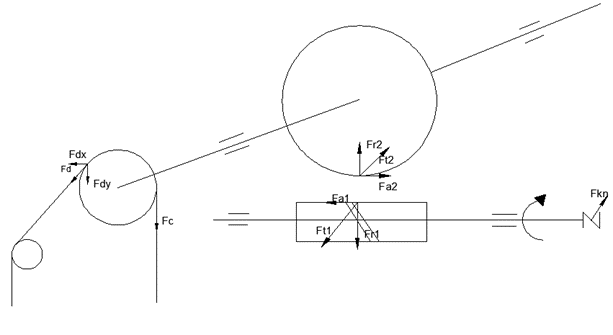
\includegraphics[width=16cm,height=9cm]{Image/force_diagram.png}}
    \caption[General force diagram]{\bfseries \fontsize{12pt}{0pt}\selectfont General force diagram}
    \label{figure1}
\end{figure}

In which:\\
- Ft1 - tangential force acting on the guide shaft I
(Ft1 is parallel to axis II, opposite rotation n1)\\
- Ft2 - tangential force acting on axis II
(Ft2 is parallel to axis I, arc of rotation n2)\\
We have the values of the forces:\\

$$F_{a1}=F_{t2}=\frac{{2\times T}_2}{d_2}=\frac{2\times593464.29}{301.5}=3936.74\left(Nmm\right)$$
$$F_{a2}=F_{t1}=\frac{2\times T_1}{d_1}=\frac{2\times7396.17}{3}=4930.78\left(Nmm\right)$$
$$F_{r1}=F_{r2}=F_{a1}\times\frac{tan\propto}{cos\gamma}=3936.74\times\frac{tan20}{cos2.08^{\circ}}=1433.67\left(Nmm\right)$$
\textbf{a.	Preliminary calculation of shaft diameter:}\\
Consider the case of full load.\\
Preliminary selection of screw diameter.
$$d_1\geq\left(0,8\ldots.1,2\right).d_{dc}=\left(0,8\ldots.1,2\right).28=\left(22,4\ldots33,6\right)mm$$
Choose d1 = 31 mm\\
Preliminary selection of worm gear diameter:
$$d_2\geq\sqrt[3]{\frac{T_2}{0,2.\left[\tau\right]}}=\sqrt[3]{\frac{1042382,5}{0,2.30}}=55,8mm,\ with τ=30 $$
Choose d2 = 60 mm\\
Look up table 10.2[I] to choose the width of the bearing:\\
			$$ b_{01} = 21 mm,  b_{02} = 31 mm	$$\\
\textbf{b.	Diagram of distance calculation for screw reducers}\\
\textbf{ Axis I} \\
Look up table 10.3[I] we have: Choose k3 = 15 mm, $h_n$ = 15 mm
$$l_{11}=d_{aM2}=304mm;l_{13}=\frac{l_{11}}{2}=\frac{304}{2}=152mm	$$
Half articulated wheel hub length :
$$l_{mkn}=l_{m12}=l_m=2.d=2.35=70mm;\;l_{12}=-l_{c12}$$
$$\bigm l_{c12}=0,5(l_{m12}+b_0)+k_3+h_n=0,5(70+21)+15+15=75,5mm$$
$$l_{12}=-l_{c12}$$
$$\bigml_{c12}=0,5(l_{m12}+b_0)+k_3+h_n=0,5(70+21)+15+15=75,5mm$$
\begin{figure}[!ht]
    \centering
     % \centerline{\includegraphics[width=1.1\textwidth, height = 1.5cm]{s_TTCD_data.png}}
   \centerline{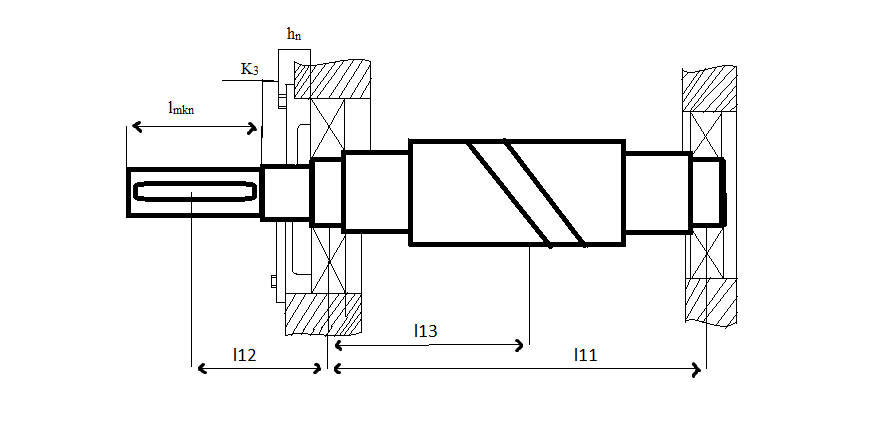
\includegraphics[width=16cm,height=9cm]{Image/axis1.png}}
    \caption[Axis II]{\bfseries \fontsize{12pt}{0pt}\selectfont Axis I}
    \label{figure1}
\end{figure}

\textbf{ Axis II} \\ 
With:
$k_1=10mm$;
$\bigmk_2=10mm$ 	
$k_3=10mm$
$\bigmh_n=15mm$
With  $	d_2 = 60 mm \rightarrow b_0=31mm$\\
\begin{figure}[!ht]
    \centering
     % \centerline{\includegraphics[width=1.1\textwidth, height = 1.5cm]{s_TTCD_data.png}}
   \centerline{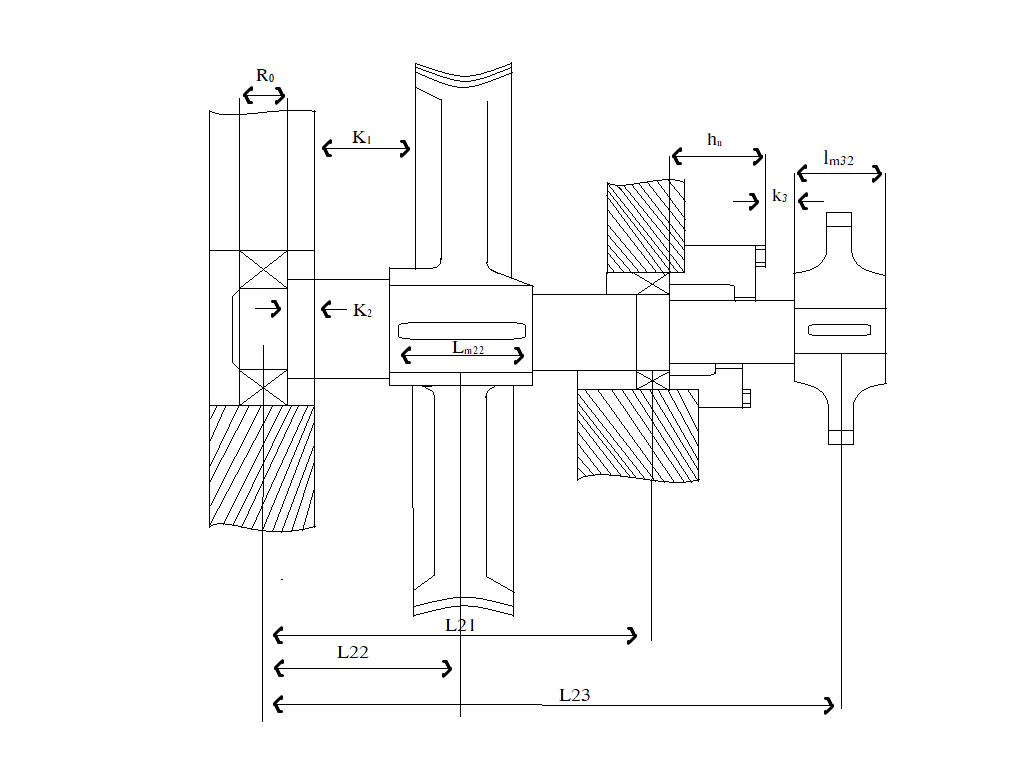
\includegraphics[width=16cm,height=9cm]{Image/axis2.png}}
    \caption[Axis II]{\bfseries \fontsize{12pt}{0pt}\selectfont Axis II}
    \label{figure1}
\end{figure}
\textbf{c. Determine the diameters and lengths of the shaft segments} 
\textbf{ Axis I}\\
Select half articulated wheel hub length $l_m = 120 mm$
\begin{figure}[!ht]
    \centering
     % \centerline{\includegraphics[width=1.1\textwidth, height = 1.5cm]{s_TTCD_data.png}}
   \centerline{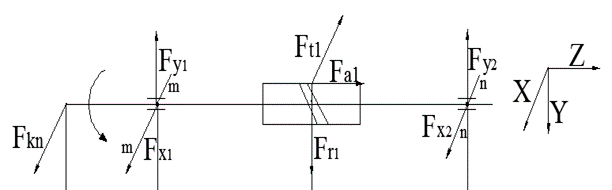
\includegraphics[width=16cm,height=5cm]{Image/Picture2.png}}
    %\caption[]{\bfseries \fontsize{12pt}{0pt}\selectfont }
    \label{figure1}
\end{figure}
We have:\\
$$M_{1x}={-F}_{r1}\times\left(I_{11}-I_{13}\right)+F_{y2}\times I_{11}-F_{a1}\times\frac{d_1}{2}=0$$
$$F_{y2}=\frac{F_{r1}\times\left(I_{11}-I_{13}\right)+F_{a1}\times\frac{d_1}{2}}{I_{11}}=\frac{2643,11\times152+7238,763\times\frac{70,4}{2}}{304}=2159,7275N$$
$$F_{y1}=F_{r1}-F_{y2}=2643,11-2159,7275=483,382N$$
$$M_{1y}=F_{t1}\times I_{13}+F_{kn}{\times I}_{12}-F_{x2}\times2\times I_{13}=0$$
$$F_{x2}=\frac{F_{t1}.\times+F_{kn}\times I_{12}}{2.I_{13}}=\frac{698,397\times152+617,626\times75}{304}=501,5733(N)$$
$$F_{x1}=F_{kn}+F_{x2}-F_{t1}=617,626 + 501,5733 -698,397=420,8023 N$$
\textbf{d.	Calculate the bending moment at the cross-sections}
$$	M_j=\sqrt{{M_{yj}}^2+{M_{xj}}^2}$$
Consider cross section m – m at 1 :\\
$$M_{mx}=F_{y2}\times I_{13}= 2159,7275\times152=328278(Nmm)$$
$$M_{my}=F_{x2}\times I_{13}=501,5733.152=76239,1416\left(Nmm\right)$$
$$M_m=\sqrt{M_{mx}^2+M_{my}^2}=\sqrt{{328278}^2+{76239,14}^2}=337014,6165\left(Nmm\right)$$
With T1 = 26189,92 (Nmm)
$$M_{td}=\sqrt{M_m^2+0,75\times T_1^2}=\sqrt{{337014,61}^2+{0,7\times.26189,92}^2}=337776,96\left(Nmm\right)$$
Consider the section n – n at 2:
$$M_{nx}=0;M_{ny}=F_{kn}.I_{12}=617,62.75=46321,5\ (Nmm)$$
$$\rightarrow M_n=M_{ny}=46321,5 (Nmm)$$
\textbf{e.	 Calculate shaft diameter at 2 sections}\\
At the cross section m - m: taken by the diameter of the screw thread foot :\\
$d_{m-m} = 70,4 mm$\\
At the cross section n - n :
$$d=\sqrt[3]{\frac{M_{td}}{0,1\left[\sigma\right]}}=\sqrt[3]{\frac{337776,96}{0,1.55}}=39,45$$
With $[\sigma]=55$ check table 10.5 shaft material made of 45 tempered steel.\\
 Choose $\Rightarrow d = 24 mm$\\
	 Choose the diameter of the fitting place to be d = 31 mm\\
	The diameter at the n – n section is taken no more than 5 mm larger than the diameter of the fitting, so choose d= 36 mm.\\
\subsection{Calculation of bearing selection for shaft I}
Select bearing type, calculate Fr at the supports 1 and 2
$$F_{r1}=\sqrt{{F^2}_{x1}+{F^2}_{y1}}=\sqrt{{420,80}^2+{483,38}^2}=640,884N$$
$$F_{r2}=\sqrt{{F^2}_{x2}+{F^2}_{y2}}=\sqrt{{501,57}^2+{2159,72}^2}=2217,19N$$
$$F_{at}=7238,77N$$
Consider $ \frac{F_{at}}{F_{r2}}=\frac{7238,77}{2217,19}=3,26$\\
For screw shafts, it is mandatory to use tapered roller bearings and at the same time, the screw shaft must arrange bearings as follows:\\%chen hinh vao
\textbf{Including:}\\
A bearing "1" so that the screw can move axially to avoid curvature of the screw due to thermal expansion.\\
A pair of "2" double tapered roller bearings that fix the shaft.\\
	Select bearing precision grade : accuracy grade 0\\
\subsubsection{Select the bearing type: single row ball bearing }
Look up table P2.7 T.254[I] We have the symbol of a light-weight single row ball bearing :208\\
We have :\\
Inner diameter d = 40 mm\\
Outer diameter D = 80 mm\\
Dynamic load capacity C = 25.6 kN\\
Calculation load capacity C0 = 18.1 kN\\
Experimental coefficient: $1.5\times \tan \alpha=1.5\times \tan10.83= 0.29$  \\
Test the load capacity of the drive\\
We have : $Q=(X.V.F_{r1}+YF_a).k_t.k_d$
In which, for ball bearings bearing radial force X = 1\\
Bearing bearing does not bear axial force, so Y = 0\\
The inner ring of the bearing rotates so V = 1\\
Factor taking into account the effect of temperature kt = 1 (because t$\le100^0c)$\\
light impact load characteristics kd = 1
$$\rightarrow Q=F_{r1}\times k_d\times k_t=640,884\times1\times1=640,89\ N$$
$$L=\frac{60\times n\times L_h}{{10}^6}=\frac{60\times1425\times12000}{{10}^6}=1026 \;( million\; revolutions) $$
Where: n is the number of shaft revolutions (rpm)\\
$Lh$ is the lifespan (hours)\\
Dynamic load capacity required with rolling bearing:\\
$$C_d^{yc}=Q\times L^\frac{1}{3}=640,884\times{1026}^\frac{1}{3}=6463,9\ N\ \approx4,46\ kN\ $$
$\Rightarrow{C_d}^{yc}<C=37,8kN $ (satisfied)
\subsubsection{Calculation of choosing a tapered roller bearing}
	 Choose a wide-range single-row tapered roller bearing with:\\
		Symbol: 7609\\
		Dynamic load capacity: C = 104 kN\\
        Static load capacity: C0 = 90.5 kN\\
        $\alpha=11^0 $\\
    Draw a bearing diagram ( using O bearings).
\begin{figure}[!ht]
    \centering
     % \centerline{\includegraphics[width=1.1\textwidth, height = 1.5cm]{s_TTCD_data.png}}
   \centerline{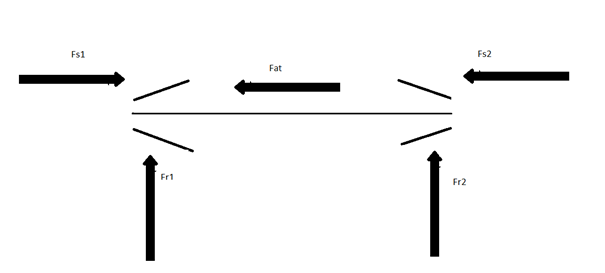
\includegraphics[width=16cm,height=7cm]{Image/Picture3.png}}
    %\caption[]{\bfseries \fontsize{12pt}{0pt}\selectfont }
    \label{figure1}
\end{figure}
Calculate e:\\
$$e=1.5\times \tan \alpha=1.5\times \tan10.83= 0.29$$
According to (11.7) axial force due to radial force on rolling bearings:\\
$$F_{s1}=F_{s2}=0,5\times0,83\times e\times F_{r2}=0,5\times0,83\times0,29\times2217,19
=266,84\ (N) $$
( For screw Fr =0,5 Fr2)\\
Calculate $ \sum F_{a1};\sum F_{a2}$
$$\sum{F_{a1}=\left|F_{s2}+F_{at}\right|=\left|266,84+7238,77\right|=7505,61\ (N)}$$
$$\sum{F_{a2}=\left|F_{s2}-F_{at}\right|=\left|266,84-7238,77\right|=-6971,93\ (N)}$$
Calculate $ F_{a1};F_{a2}$\\
$$F_{a1}=Max(F_{s1};\sum{F_{a1})=7505,61}$$
$$F_{a2}=Max(F_{s2};\sum{F_{a2})=6971,93}$$
Calculate Q1; Q2 (conventional dynamic load)\\
	Consider $ \ \frac{F_{a1}}{0,5\times V\times F_{r2}}=\frac{7505,61}{0,5\times2217,19}=6,77$ > e, so:\\
	X1 = 0,4; Y1 = 0,4.cotg110 = 2,06
$$	\Rightarrow Q_1=(X.V.F_{r1}+YF_{a1}).k_t.k_d$$
$$ =\left(0,4\times0,5\times2217,19+2,06\times7505,61\right)\times1\times1$$
$$=15904,99\ (N)$$
Dynamic load testing:\\
Q = Max(Q1,Q2) = Q1 = 15904,99 N\\
$$L=\frac{60\times n\times L_h}{{10}^6}=\frac{60\times1425\times12000}{{10}^6}=1026 \; ( million\; revolutions)$$
Dynamic load capacity required for rolling bearing:\\
$$C_d^{yc}=Q\times L^\frac{3}{10}=15904,99\times{1026}^\frac{3}{10}=127314,43\ N\ \approx127,31\ kN\ $$
${C_d}^{yc}>C $ unsatisfactory\\
We reduce the bearing life: every $\frac{L_h}{3}$ then change the bearing 1 time.\\
 Therefore : $L = \frac{1026}{3}=342$
 $${\rightarrow C}_d^{yc}=Q\times L^\frac{3}{10}=15904,99\times{342}^\frac{3}{10}=91567,47\ N\ \approx91,56\ kN\ $$
$ {C_d}^{yc}<C=104(kN) $ satisfied
\subsection{Preliminary calculation of shaft diameter II and roller bearing II}
\subsubsection{Determine the preliminary diameter}
$$d_{2sb}=3TII0,2[τ] pick [\tau]=22÷28>[τ] axis I \Rightarrow[\tau]=25$$
$\Rightarrow d_{2sb}=\sqrt[3]{\frac{1043282,5}{0,2.25}}=59,3 (mm) $ => choose $d_{2sb}$  = 60 mm\\
Choose $d3 <d2sb \Rightarrow $ choose d3  = 55 mm\\
d0 = d2sb = 60 mm\\
d1 > d0 choose d1 = 65 mm\\
Draw the shaft texture:\\
\begin{figure}[!ht]
    \centering
     % \centerline{\includegraphics[width=1.1\textwidth, height = 1.5cm]{s_TTCD_data.png}}
   \centerline{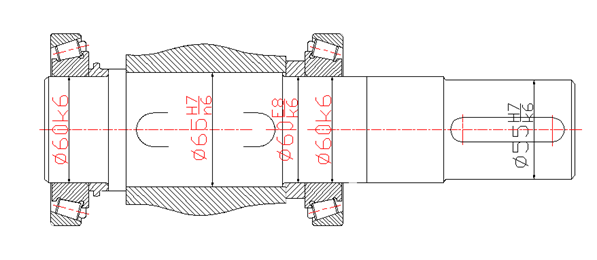
\includegraphics[width=16cm,height=7cm]{Image/Picture4.png}}
    %\caption[]{\bfseries \fontsize{12pt}{0pt}\selectfont }
    \label{figure1}
\end{figure}
\subsubsection{Select the bearing at the 0 and 2 buttons}
Choose a light-sized 7612 tapered roller bearing with d = d0 = 60 mm\\
Tapered roller bearing has D = 130 mm; B = 46 mm\\
\section{Structural calculation of the speed reduction box}
\subsection{Worm gear texture}
From the picture 14-14t.16[II] and the formulas we have:\\
	Shaft distance a = 190 mm ,\\
	Width of worm gear b2 = 60 mm ,\\
	Sewing length lm  = 90 mm\\
	Tilt angle $\gamma$ = 5,710\\
	Diameter of top ring d a2  = 292,92 mm \\
	Diameter of dividing ring d2  = 285 mm \\
	Diameter of bottom ring df2 = 279,72 mm \\
\subsection{Screw structure }
\subsection{Gearbox structure }
- The standard of the reducer housing is high rigidity and small weight. \\
- Choosing the material for casting the reducer is gray cast iron with the symbol GX 15-32. \\
- Choose a mounting surface that passes through the center of the shaft and the body for easy mounting.  \\
Basic sizes\\
